% final_report.tex
\documentclass[12pt,a4paper]{article}
\usepackage[margin=1in]{geometry}
\usepackage{amsmath,amssymb}
\usepackage{graphicx}
\usepackage{booktabs}
\usepackage{float}
\usepackage{hyperref}
\usepackage{listings}
\usepackage{xcolor}

% Listings style
\lstset{
language=Python,
basicstyle=\ttfamily\small,
breaklines=true,
frame=single,
backgroundcolor=\color{gray!10},
showstringspaces=false
}

\title{Pricing Exotic Options using Stochastic Calculus, PDEs, and Monte Carlo Simulations}
\author{Ajay Singh \\ ajay.s.works@gmail.com}
\date{June 2025}

\begin{document}
\maketitle

\begin{abstract}
This report presents a computational framework for pricing exotic options, integrating stochastic calculus, Monte Carlo simulations, and finite difference PDE methods. We implement and validate each method on vanilla and exotic derivatives, such as Asian and Barrier options, and analyze their accuracy, convergence, and runtime efficiency.
\end{abstract}
\newpage

\tableofcontents
\newpage

\section{Introduction and Literature Review}
Options are fundamental financial derivatives that grant the right, but not the obligation, to buy or sell assets. While vanilla options have well-known analytical pricing formulas, exotic options — such as Asian and Barrier options require advanced methods due to their path-dependence and complex boundary conditions.

Monte Carlo methods offer flexibility and scalability, especially for high-dimensional problems or when dealing with path-dependent payoffs. Various enhancements like antithetic variates, control variates, and quasi-Monte Carlo methods (e.g., Sobol sequences) improve convergence and reduce variance. PDE solvers like Crank-Nicolson are deterministic alternatives that provide fast and accurate results for European-style options but struggle with complex payoff structures.

The original pricing framework was introduced by Black and Scholes~\cite{black1973pricing}. Later extensions by Hull~\cite{hull2018options}, Glasserman~\cite{glasserman2004monte}, and Shreve~\cite{shreve2004stochastic} provided the foundation for Monte Carlo simulations and stochastic calculus-based techniques. This project builds upon these methods and contributes Python implementation and experimental comparison of these frameworks.

\section{Methodology}

This project adopts a modular and comparative framework for pricing exotic options, incorporating analytical formulas, stochastic simulations, and numerical PDE solvers. The methodology covers three primary engines: the Black-Scholes analytical solution, Monte Carlo simulations (with multiple variance reduction techniques), and finite difference methods for solving the Black-Scholes PDE. Each engine is validated on European options and extended to exotic options like Asian and barrier types.

\subsection{Stochastic Calculus and Black-Scholes PDE}
We implemented the closed-form Black-Scholes formula for pricing European call and put options. The analytical solution provides a benchmark to validate numerical results from other engines. We begin with the standard Geometric Brownian Motion (GBM) model for the underlying asset price and constant volatility:

\[
dS_t = \mu S_t \,dt + \sigma S_t \,dW_t,
\]

where \( \mu \) is the drift, \( \sigma \) the volatility, and \( W_t \) a standard Brownian motion. Under the risk-neutral measure \( \mathbb{Q} \), the drift becomes the risk-free rate \( r \), leading to:

\[
dS_t = r S_t \,dt + \sigma S_t \,dW_t^\mathbb{Q}.
\]

Applying Itô’s Lemma and no-arbitrage arguments yields the celebrated Black-Scholes partial differential equation (PDE):

\[
\frac{\partial V}{\partial t} + \frac{1}{2} \sigma^2 S^2 \frac{\partial^2 V}{\partial S^2} + r S \frac{\partial V}{\partial S} - rV = 0.
\]

This serves as the base PDE for analytical and numerical methods.

\begin{figure}[H]
\centering
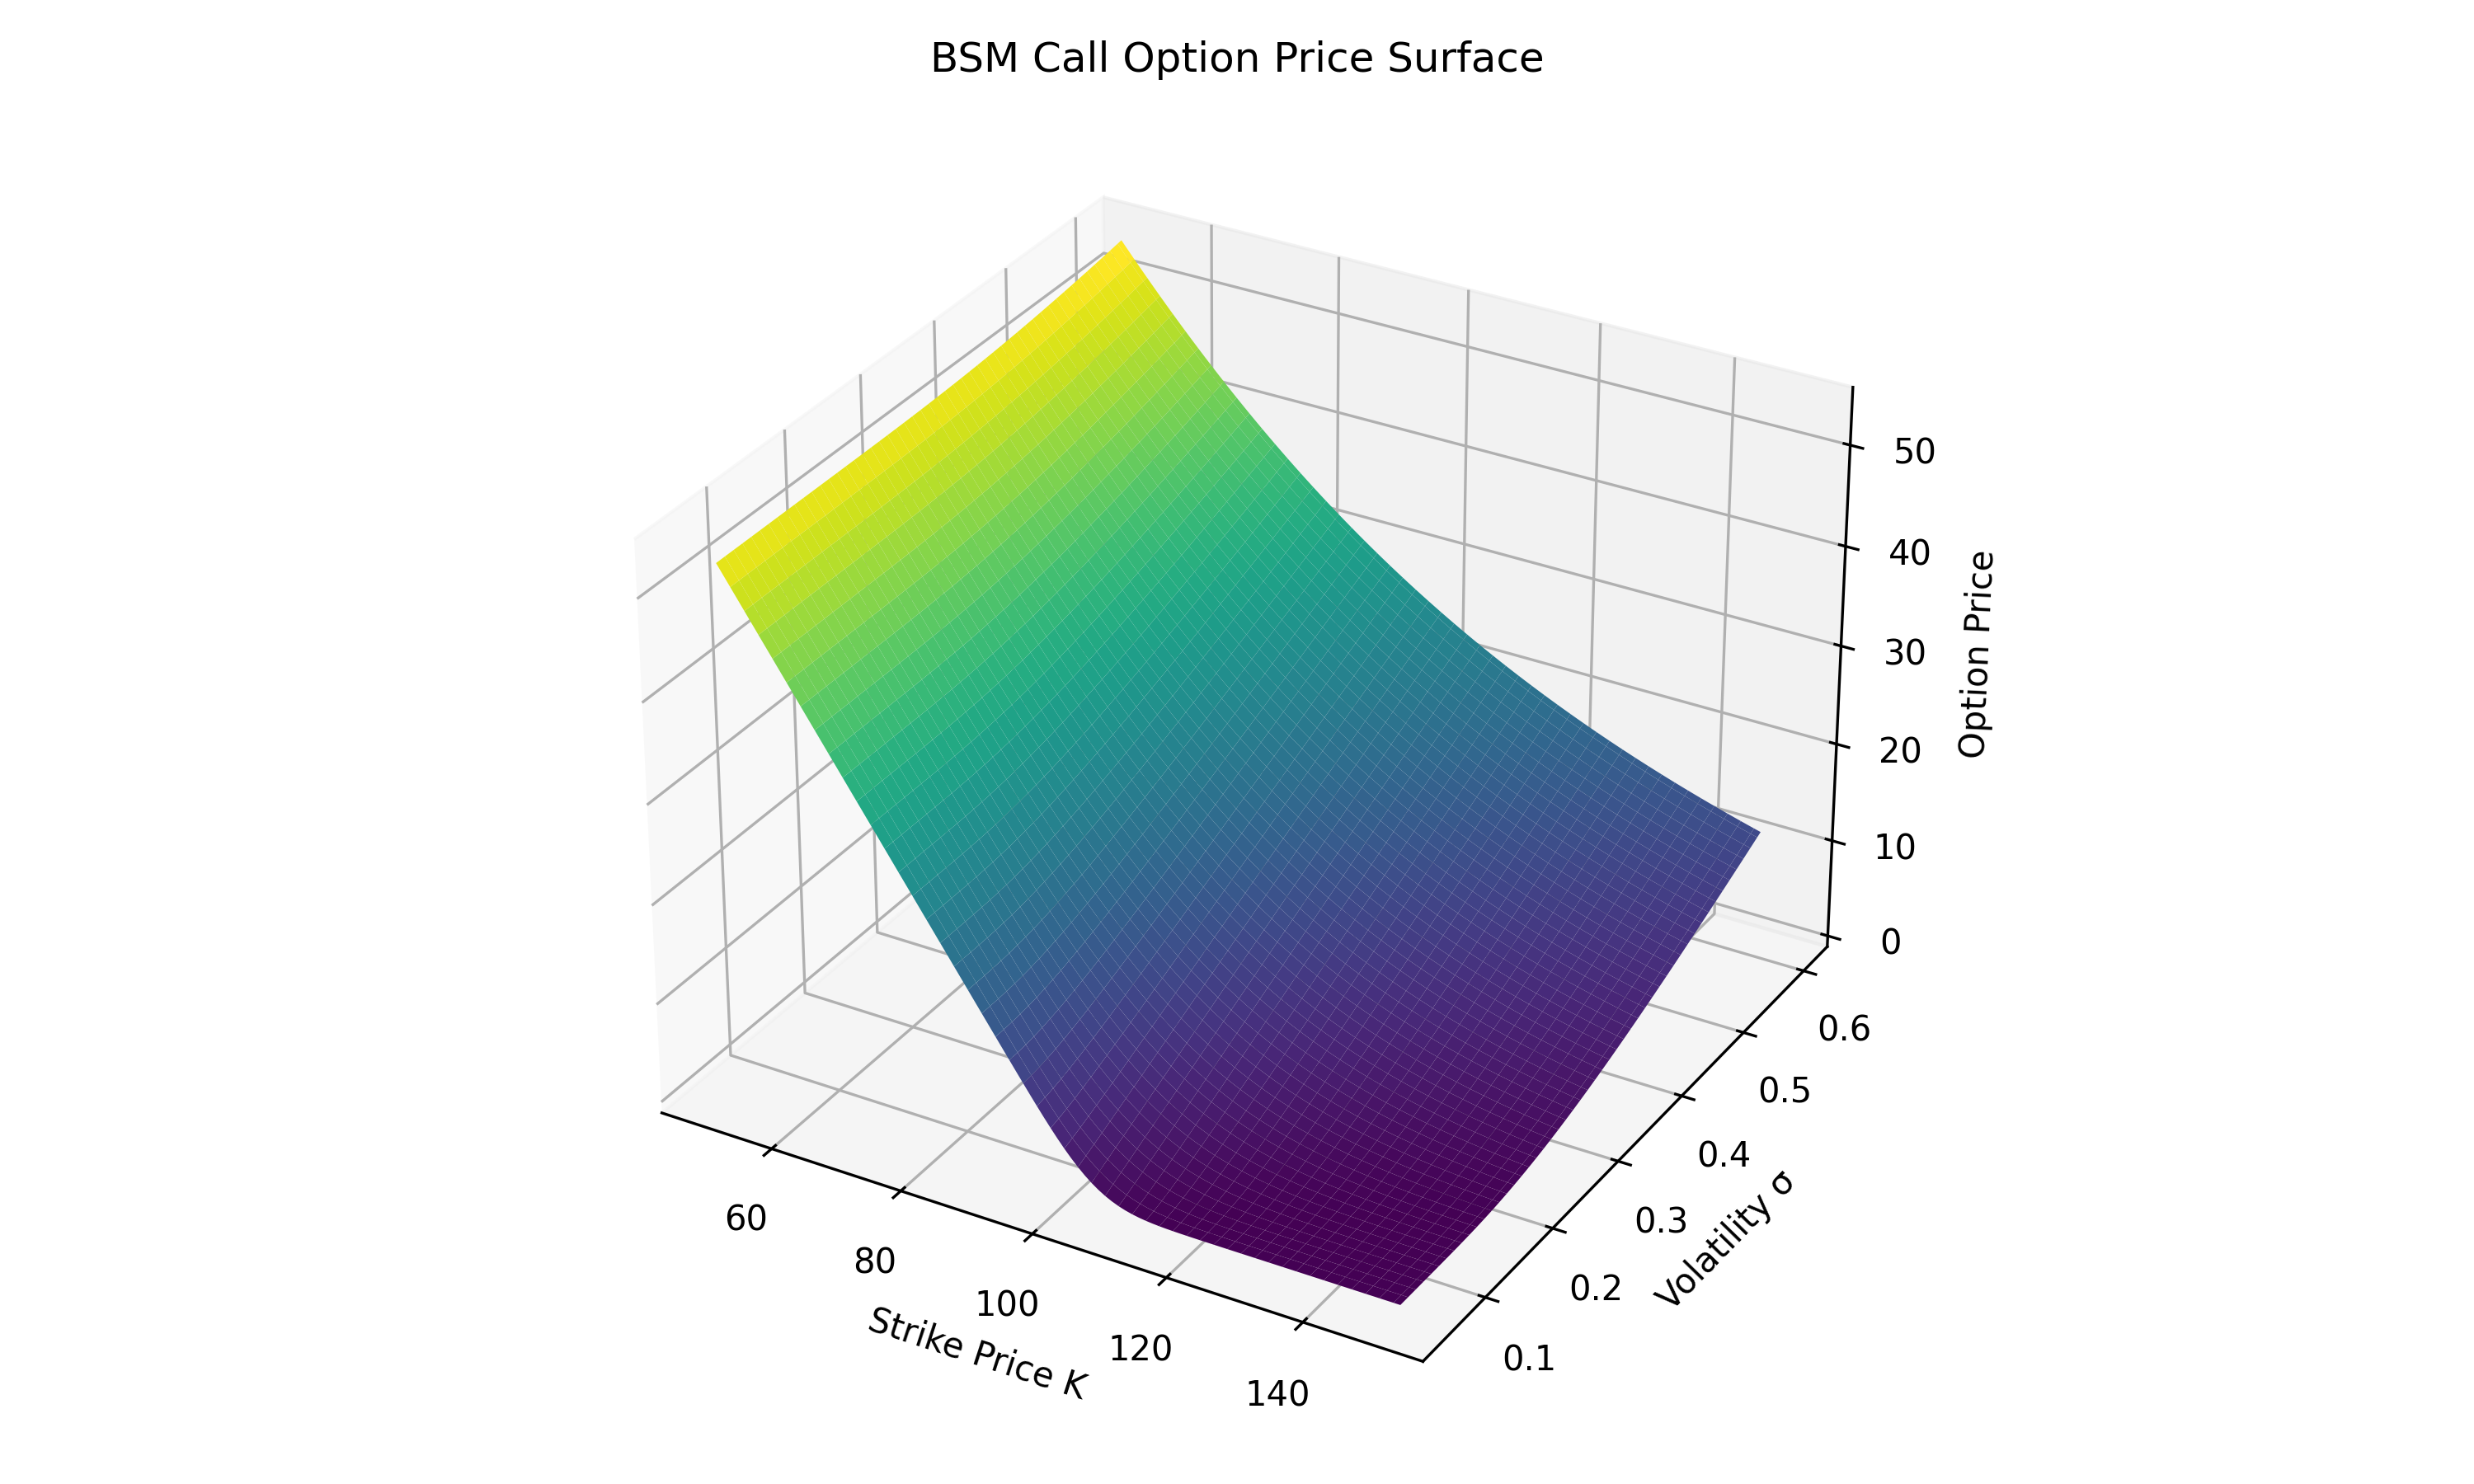
\includegraphics[width=0.7\textwidth]{../plots/bsm_surface.png}
\caption{BSM Call Option Price Surface as a function of Strike Price $K$ and Volatility $\sigma$}
\end{figure}

\subsection{Monte Carlo Simulation and Variance Reduction}
Monte Carlo (MC) simulations were employed to price both vanilla and exotic options by simulating thousands of underlying asset price paths under the risk-neutral measure. We used both Euler-Maruyama discretization and exact Brownian motion sampling. This approach naturally accommodates the pricing of path-dependent instruments, such as Asian options (which depend on average prices) and barrier options (which activate or expire based on price thresholds).

Monte Carlo (MC) simulation estimates the option value as the discounted expected payoff:

\[
V_0 = e^{-rT} \, \mathbb{E}^{\mathbb{Q}}[\text{Payoff}(S_T)],
\]

where the terminal asset price \( S_T \) is simulated using a discretized GBM scheme:

\[
S_{t+\Delta t} = S_t \exp \left[ \left( r - \frac{1}{2}\sigma^2 \right) \Delta t + \sigma \sqrt{\Delta t} Z \right],
\quad Z \sim \mathcal{N}(0,1).
\]

To enhance convergence and reduce variance, we implemented:

\begin{itemize}
  \item \textbf{Antithetic Variates}: Simulating both \( Z \) and \( -Z \) per path to reduce sampling noise.
  \item \textbf{Control Variates}: Leveraging a known European option price to adjust exotic option estimators.
  \item \textbf{Quasi-Monte Carlo}: Using Sobol sequences instead of pseudo-random numbers to achieve faster convergence.
\end{itemize}

Each method is benchmarked using convergence diagnostics and confidence intervals to assess numerical stability and efficiency.


\subsection{Finite Difference Methods (PDE)}
Finite difference methods, specifically the Crank-Nicolson scheme, are employed to numerically solve the Black-Scholes PDE. It is an implicit time-stepping scheme with second-order accuracy in both time and space. The equation is discretized as follows:

\[
\frac{V_i^{n+1} - V_i^n}{\Delta t} = \frac{1}{2} \left( \mathcal{L} V^{n+1} + \mathcal{L} V^n \right),
\]

where \( \mathcal{L} \) is the spatial differential operator defined by:

\[
\mathcal{L} V_i = \frac{1}{2} \sigma^2 S_i^2 \frac{V_{i+1} - 2V_i + V_{i-1}}{(\Delta S)^2} + r S_i \frac{V_{i+1} - V_{i-1}}{2 \Delta S} - r V_i.
\]

Boundary conditions (Dirichlet and Neumann) are applied to ensure numerical stability and meaningful solutions, particularly for options with rebate conditions or knock-out features.

\subsection{Greek Estimation and Sensitivity Analysis}
Option sensitivities, or Greeks, are essential for hedging and risk management. We compute first- and second-order Greeks using both finite difference approximations and Monte Carlo estimators:

\begin{itemize}
  \item \textbf{Delta} (\( \Delta \)) – sensitivity to the underlying price \( S \)
  \item \textbf{Gamma} (\( \Gamma \)) – rate of change of Delta
  \item \textbf{Vega} – sensitivity to volatility \( \sigma \)
\end{itemize}

These were estimated using below methods:

\begin{itemize}
    \item \textbf{Finite Difference Method:} Central differences are applied to compute Delta, Gamma, and Vega.
    \item \textbf{Pathwise Derivative Method:} Applicable to smooth payoff functions, this method computes Greeks directly along each simulated path.
    \item \textbf{Likelihood Ratio Method:} Enables estimation of sensitivities even for discontinuous payoffs, such as those in barrier options.
\end{itemize}

These estimators are validated across multiple pricing engines and are evaluated for consistency and convergence.

\subsection{Comparative Analysis Framework}

The three pricing methodologies are evaluated comparatively along several key dimensions:

\begin{itemize}
    \item \textbf{Accuracy:} Estimated prices are compared against known analytical or highly resolved numerical benchmarks.
    \item \textbf{Convergence:} Log-log convergence plots are produced for path count (MC) and grid resolution (PDE).
    \item \textbf{Computational Efficiency:} Runtime vs. error trade-offs are analyzed across pricing engines.
    \item \textbf{Robustness:} Performance is assessed on exotic options with path-dependent features, to reveal limitations and strengths of each approach.
\end{itemize}

This systematic and extensible methodology facilitates not only cross-validation of numerical methods but also provides a platform for testing novel variance reduction and hedging techniques in future work.

\section{Experiments and Results}

This section presents the empirical evaluation of various numerical methods implemented for pricing vanilla and exotic options. The experiments cover accuracy, convergence behavior, computational efficiency, and sensitivity to input parameters. Results were obtained under consistent model assumptions, with careful calibration and validation against analytical solutions where available.

\subsection{Experimental Setup}

We consider European, Asian, and Barrier options under the standard Black-Scholes framework. The baseline parameters used across simulations are:
\begin{itemize}
    \item Initial asset price: $S_0 = 100$
    \item Strike price: $K = 100$
    \item Risk-free rate: $r = 5\%$
    \item Volatility: $\sigma = 20\%$
    \item Time to maturity: $T = 1$ year
\end{itemize}

\subsection{Convergence Behavior of Monte Carlo Simulations}

We begin by evaluating the convergence behavior of the Monte Carlo (MC) method for vanilla options. As expected, the error follows a $\mathcal{O}(1/\sqrt{N})$ trend.

\begin{figure}[H]
    \centering
    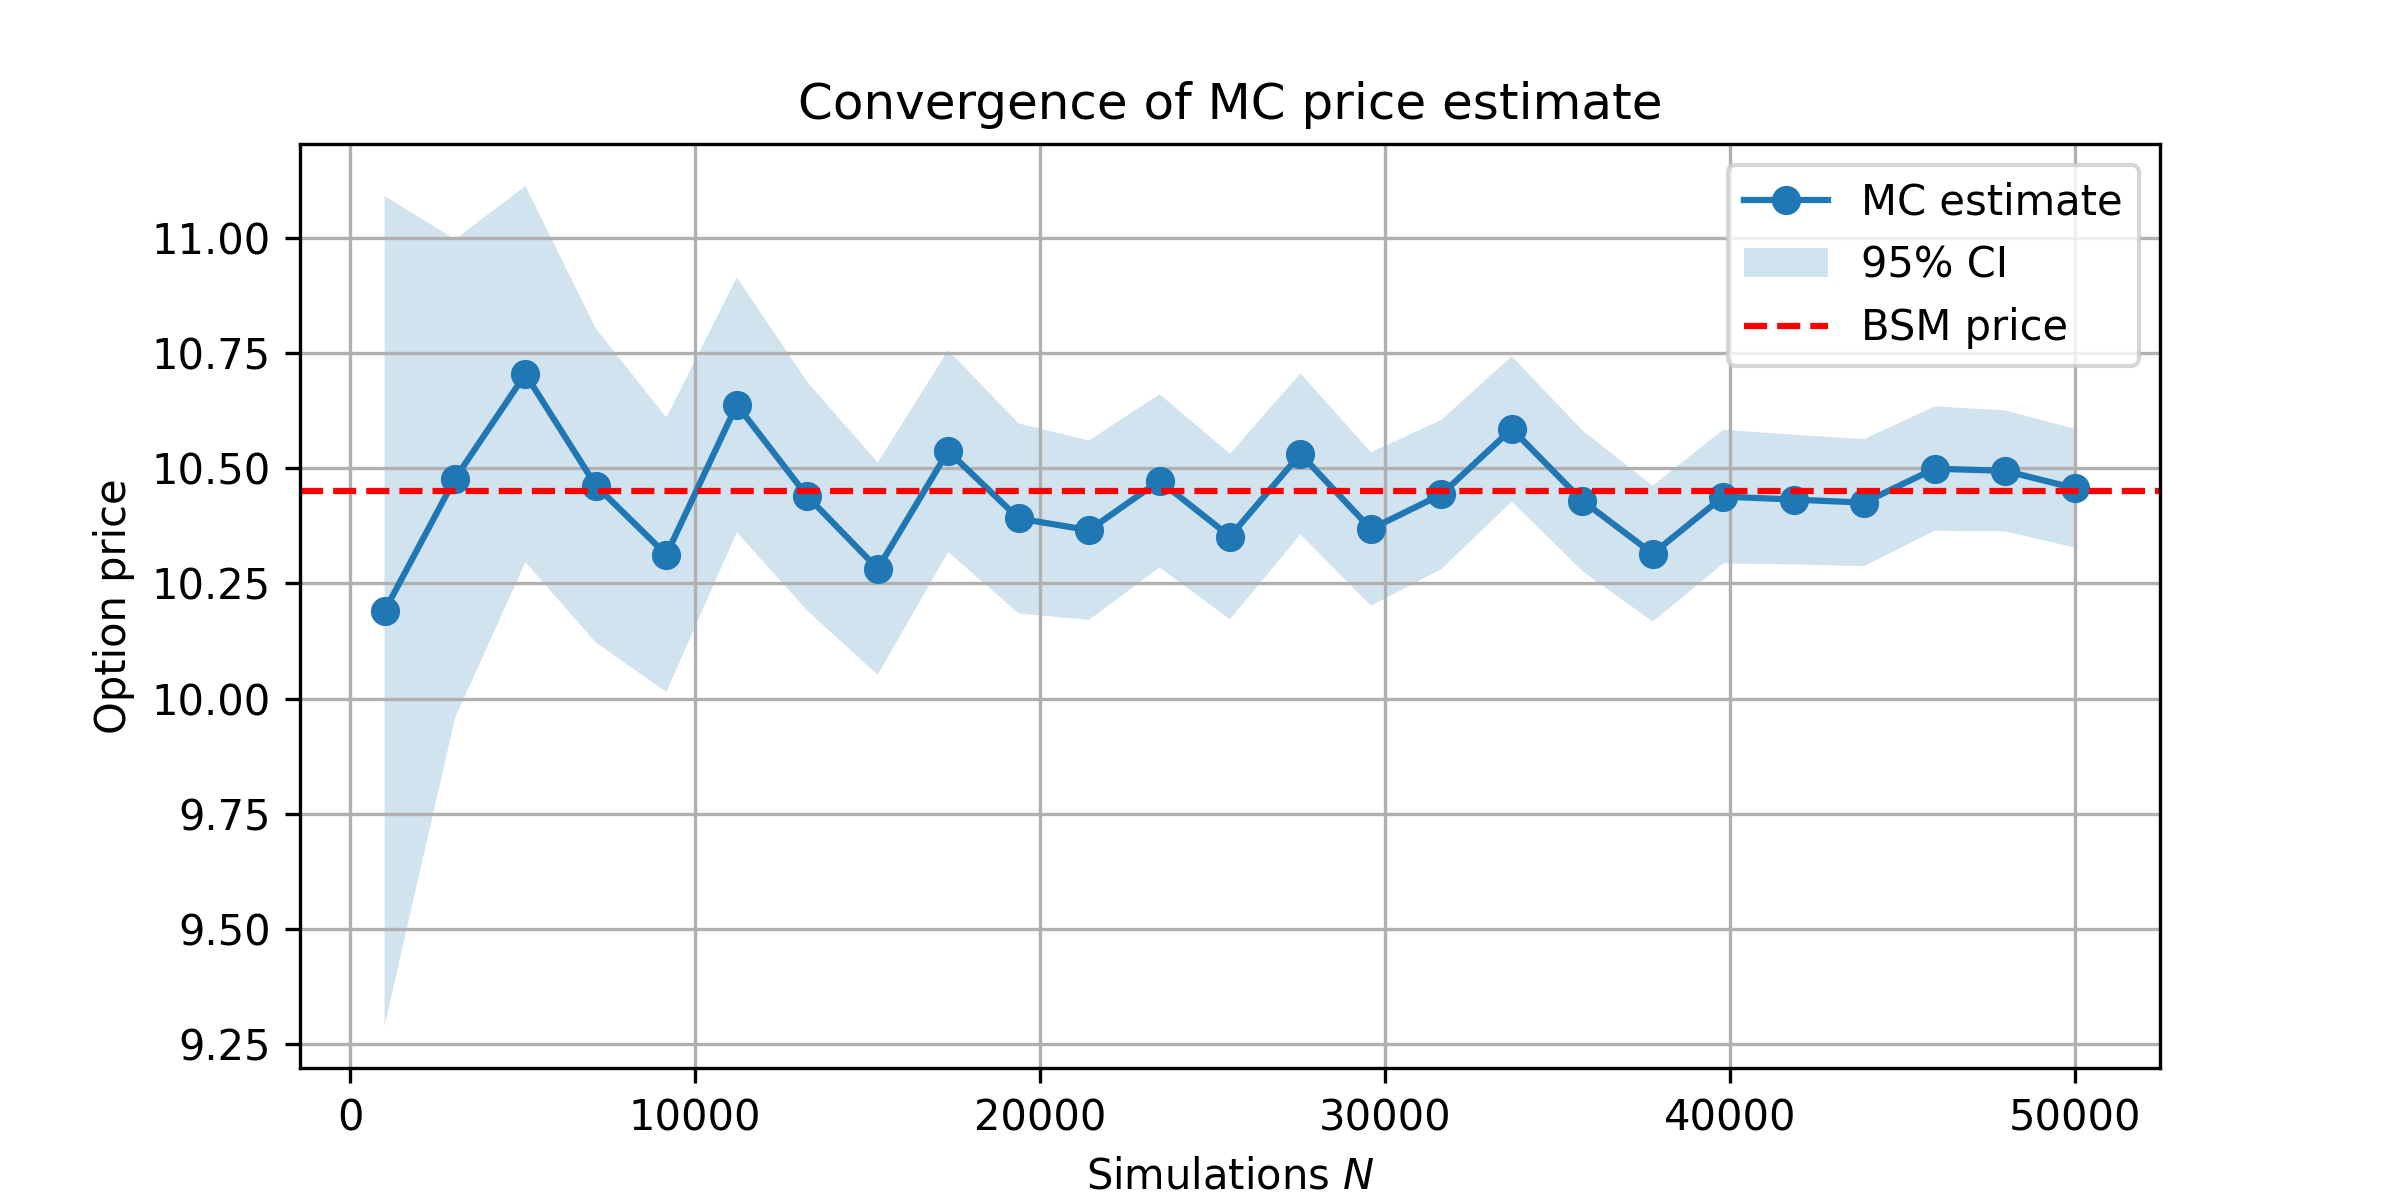
\includegraphics[width=0.7\textwidth]{../plots/mc_convergence.png}
    \caption{Convergence of Monte Carlo estimates with increasing number of simulations. Error decreases proportionally to $1/\sqrt{N}$, as theoretically expected.}
\end{figure}

\subsection{Comparative Convergence: Binomial, PDE, and Monte Carlo}

To better understand the accuracy across schemes, we compare the convergence behavior of MC, finite-difference PDE, and binomial tree methods. All were benchmarked against BSM closed-form solutions.

\begin{figure}[H]
    \centering
    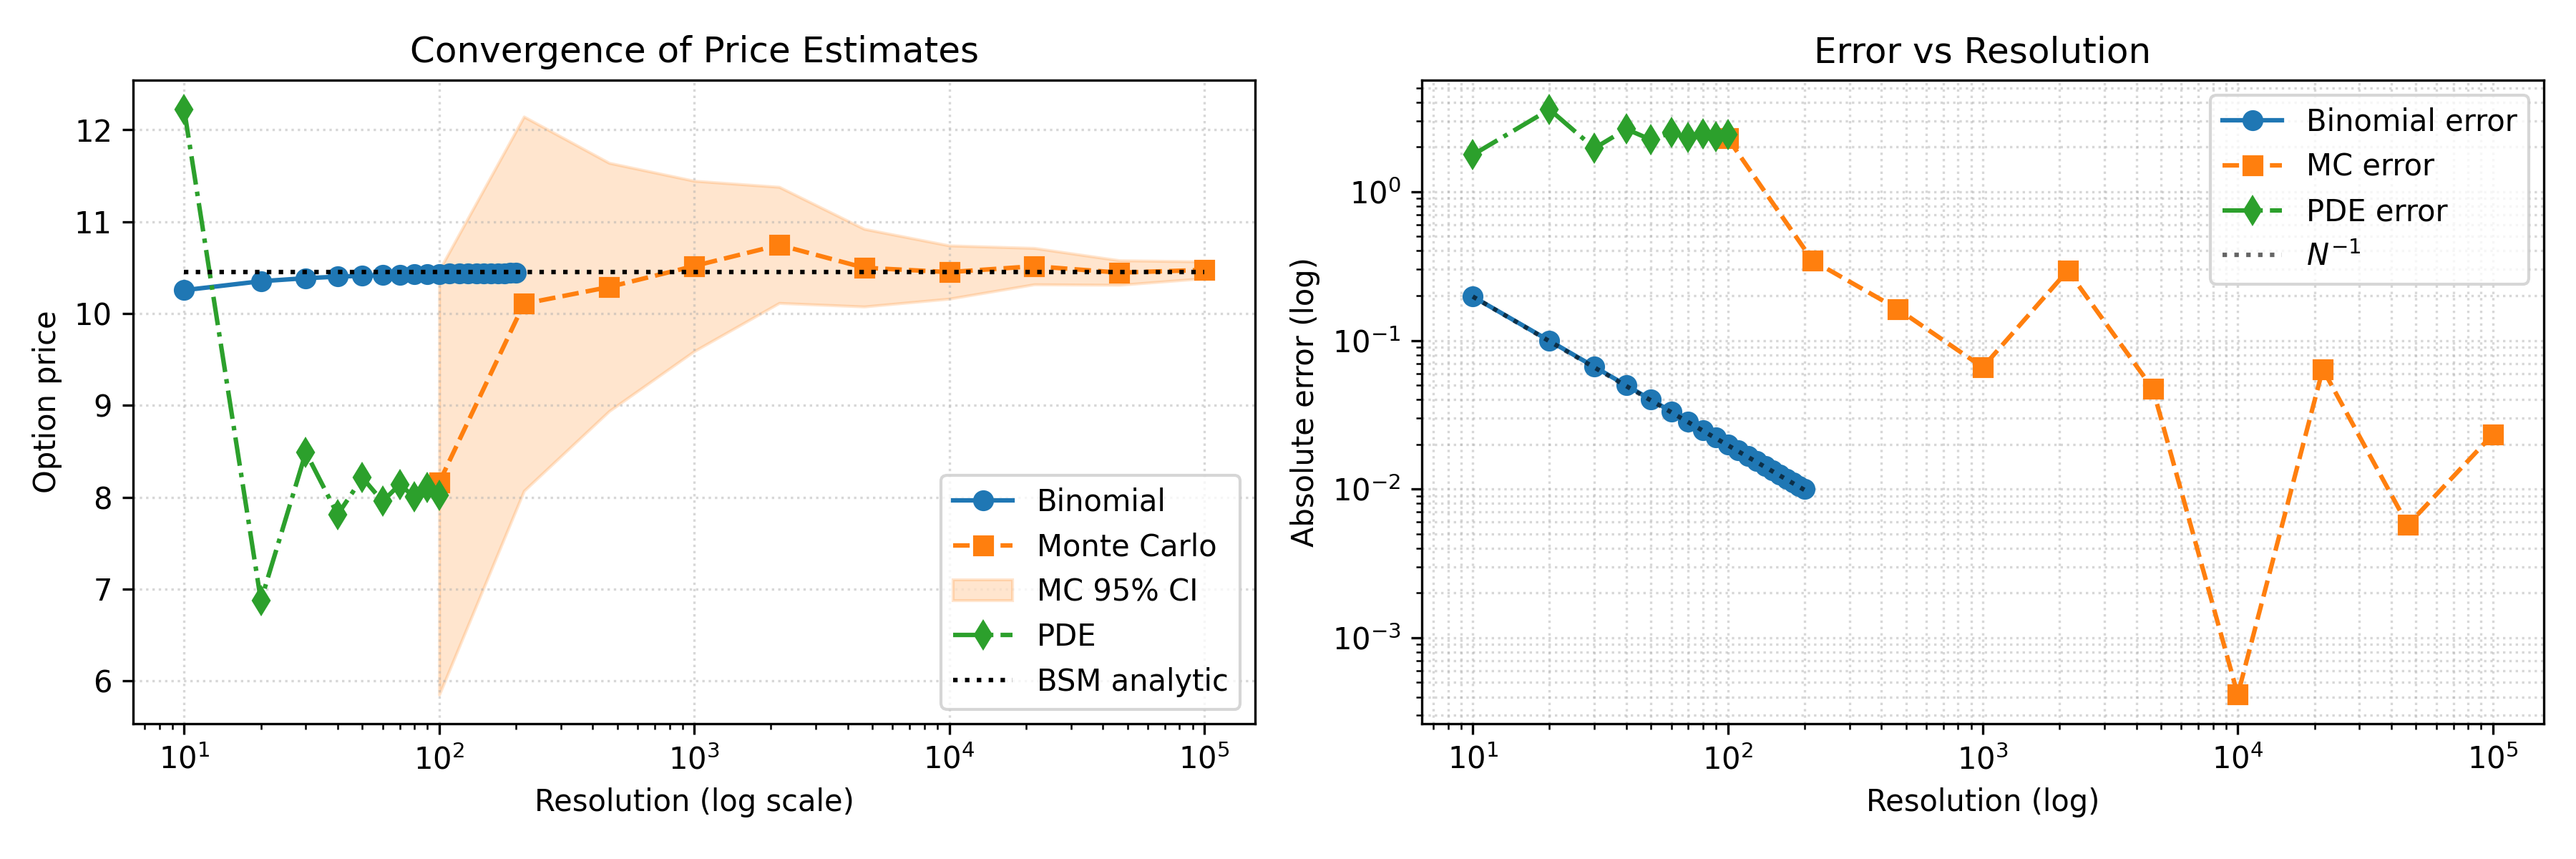
\includegraphics[width=0.95\textwidth]{../plots/mc_pde_binomial_convergence.png}
    \caption{Convergence of Binomial, Monte Carlo, and PDE methods for European call pricing. PDE achieves faster convergence with fewer grid steps; Binomial is consistent but slower; MC exhibits high variance at lower sample sizes.}
\end{figure}
\vspace{-5mm}

\subsection{Convergence of PDE Solvers}

We further examine the stability and convergence of the Crank–Nicolson finite-difference method.

\begin{figure}[H]
    \centering
    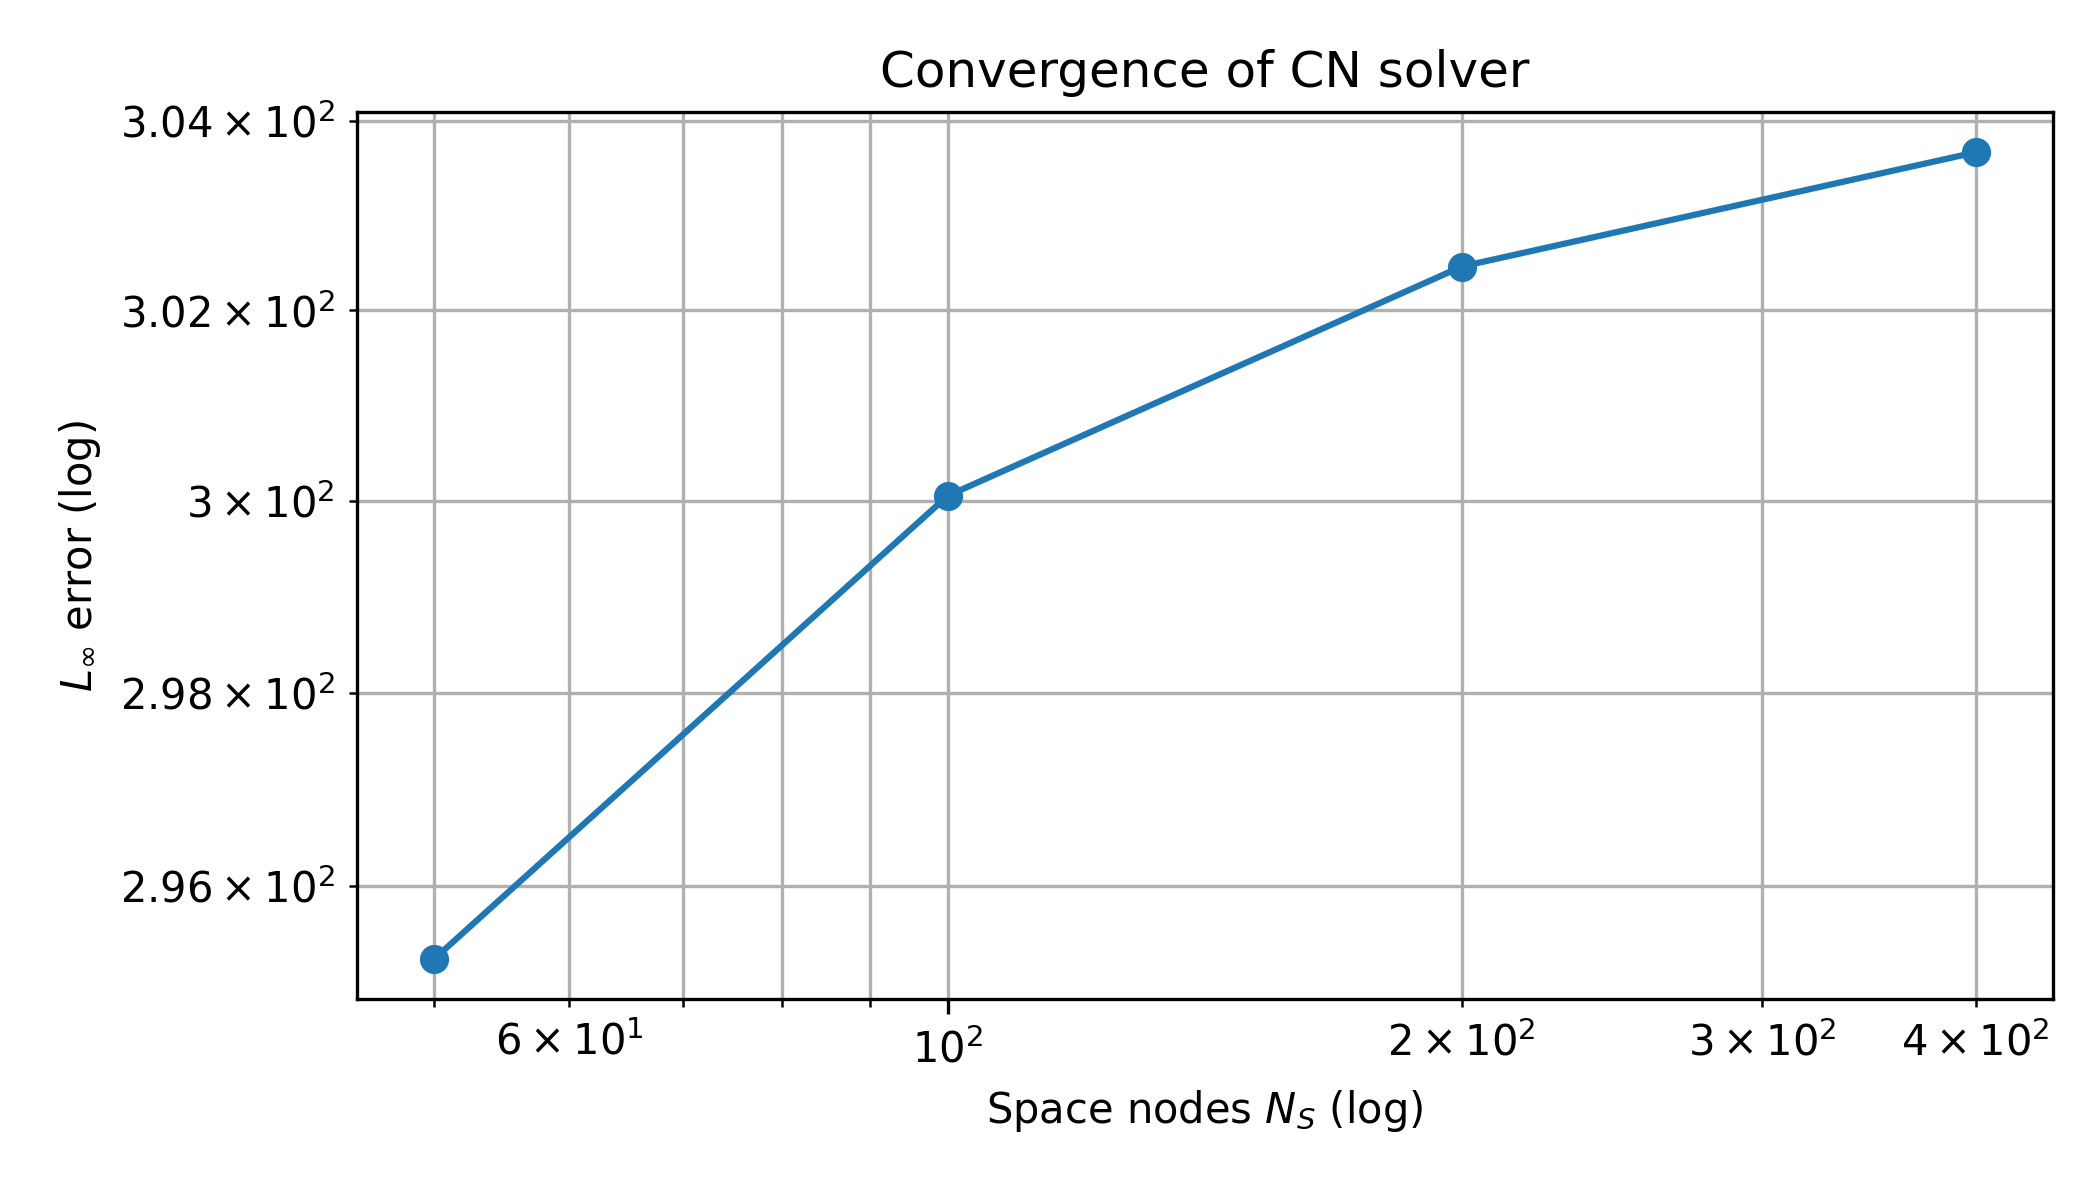
\includegraphics[width=0.8\textwidth]{../plots/PDE_convergence.png}
    \caption{Convergence of the PDE method using Crank–Nicolson discretization. The results align well with theoretical second-order accuracy in time and space.}
\end{figure}
\newpage

\subsubsection{Comparison of BSM, Monte Carlo, and PDE Pricing}

We compare the option prices obtained via the Black-Scholes-Merton (BSM) analytical formula, Monte Carlo simulations, and the Crank-Nicolson finite difference method.

\begin{figure}[H]
    \centering
    \includegraphics[width=0.6\textwidth]{../plots/BSM_MC_CN_Comparison.png}
    \caption{Comparison of vanilla option prices using BSM analytical formula, Monte Carlo simulation, and Crank-Nicolson PDE method. The prices align closely, validating cross-method consistency.}
    \label{fig:bsm_mc_cn_comparison}
\end{figure}

\subsection{Exotic Option Pricing Comparison}

We benchmark pricing of exotic instruments (barrier and Asian options) against reference methods.

\begin{figure}[H]
    \centering
    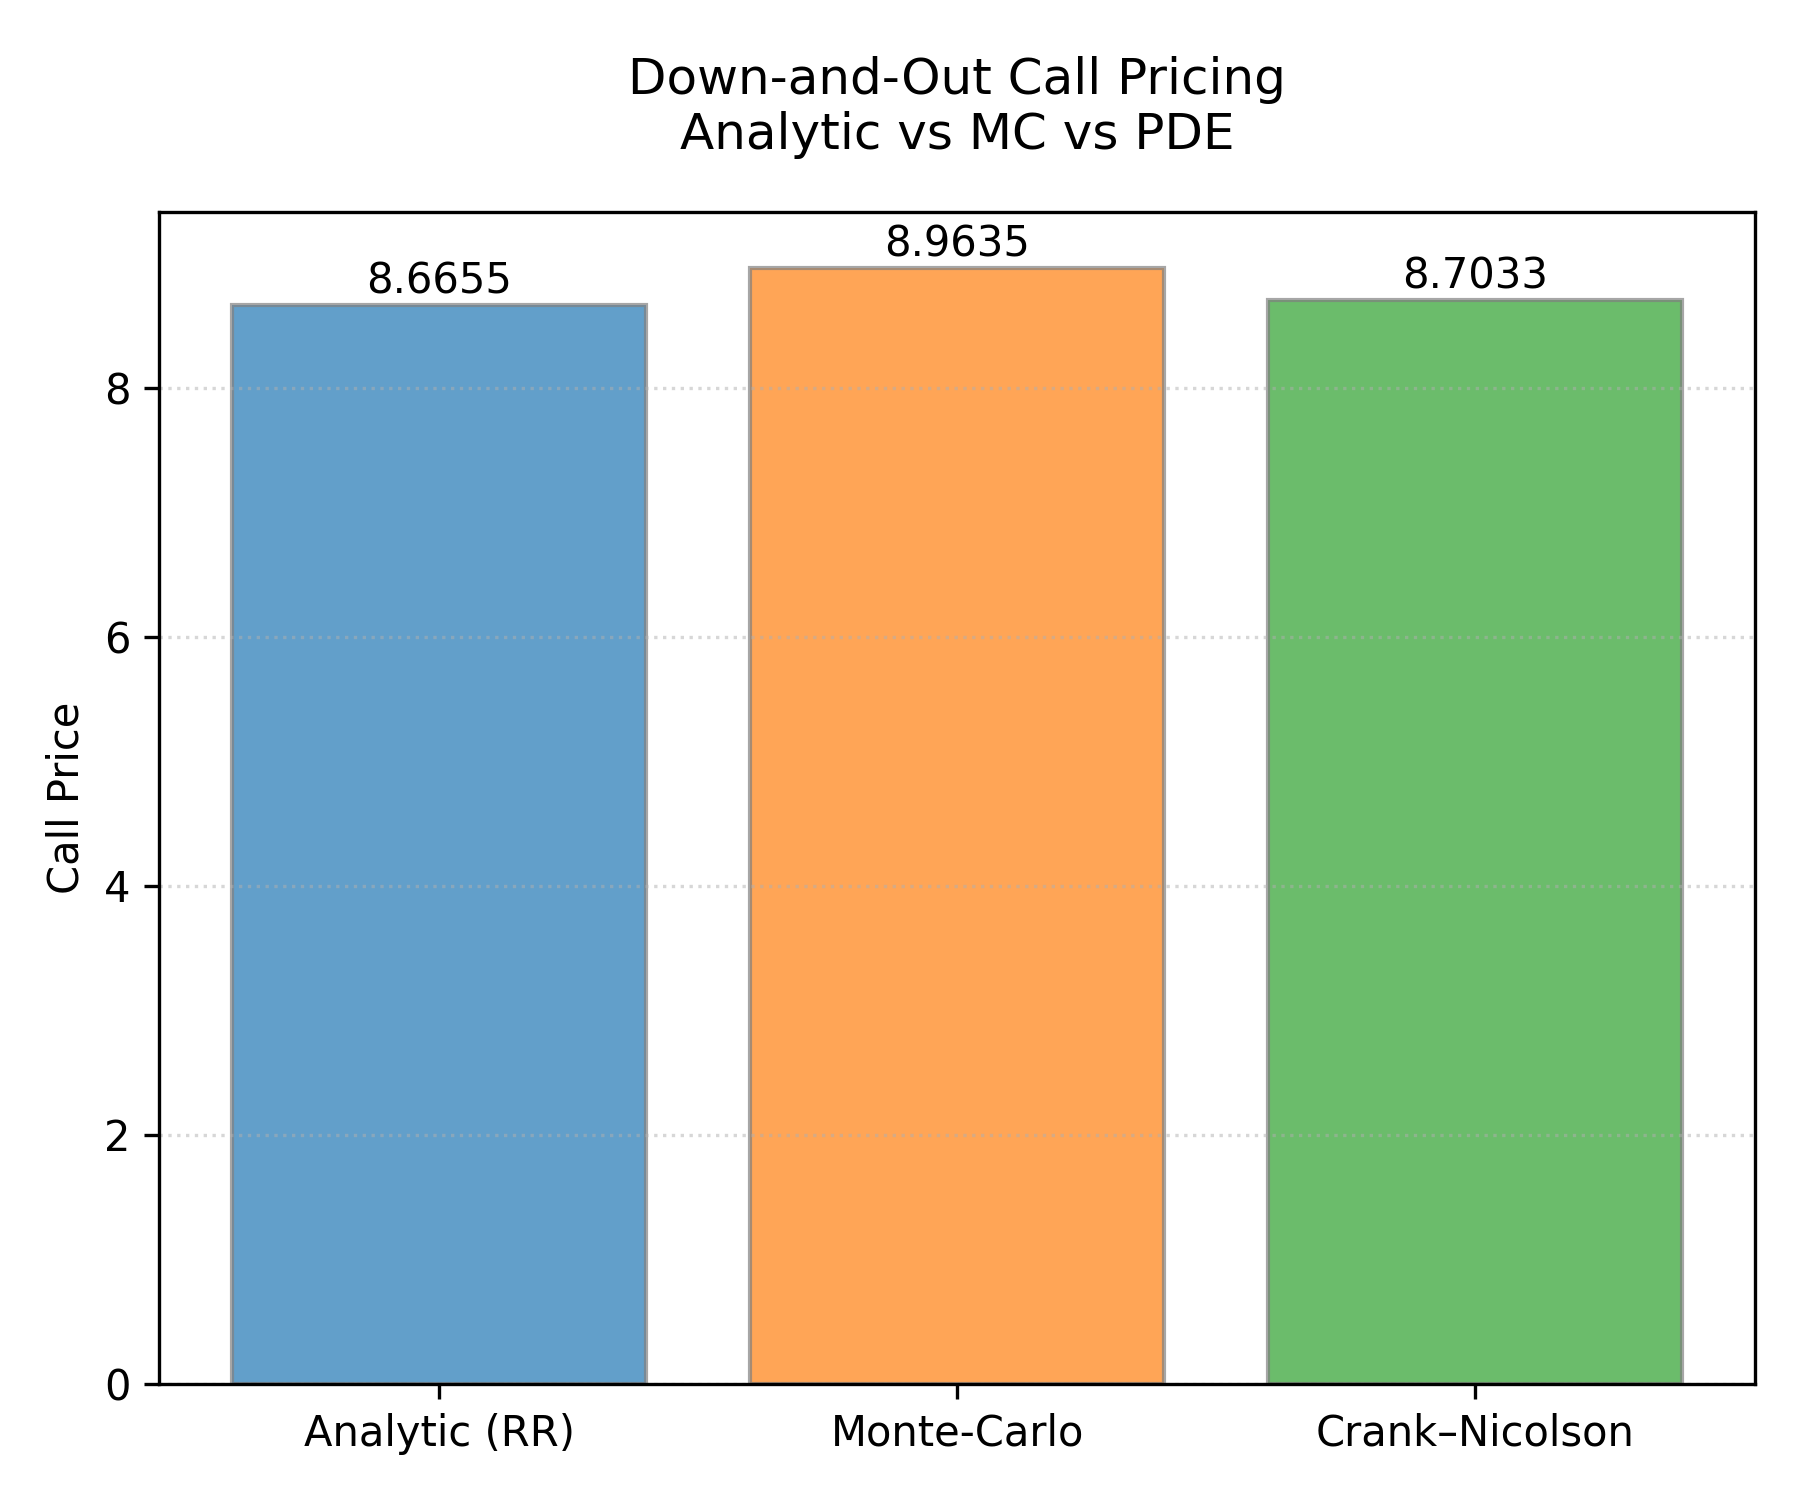
\includegraphics[width=0.6\textwidth]{../plots/barrier_price_compare.png}
    \caption{Comparison of up-and-out barrier option pricing using MC with and without variance reduction techniques. Accuracy improves with control and antithetic variates.}
\end{figure}
\newpage

\subsection{ADI Method for Asian Option Pricing}

The Alternating Direction Implicit (ADI) Crank–Nicolson scheme was applied to price arithmetic Asian options. The following convergence plot highlights the performance of the spatial and temporal discretization in the PDE framework.
\begin{figure}[H]
    \centering
    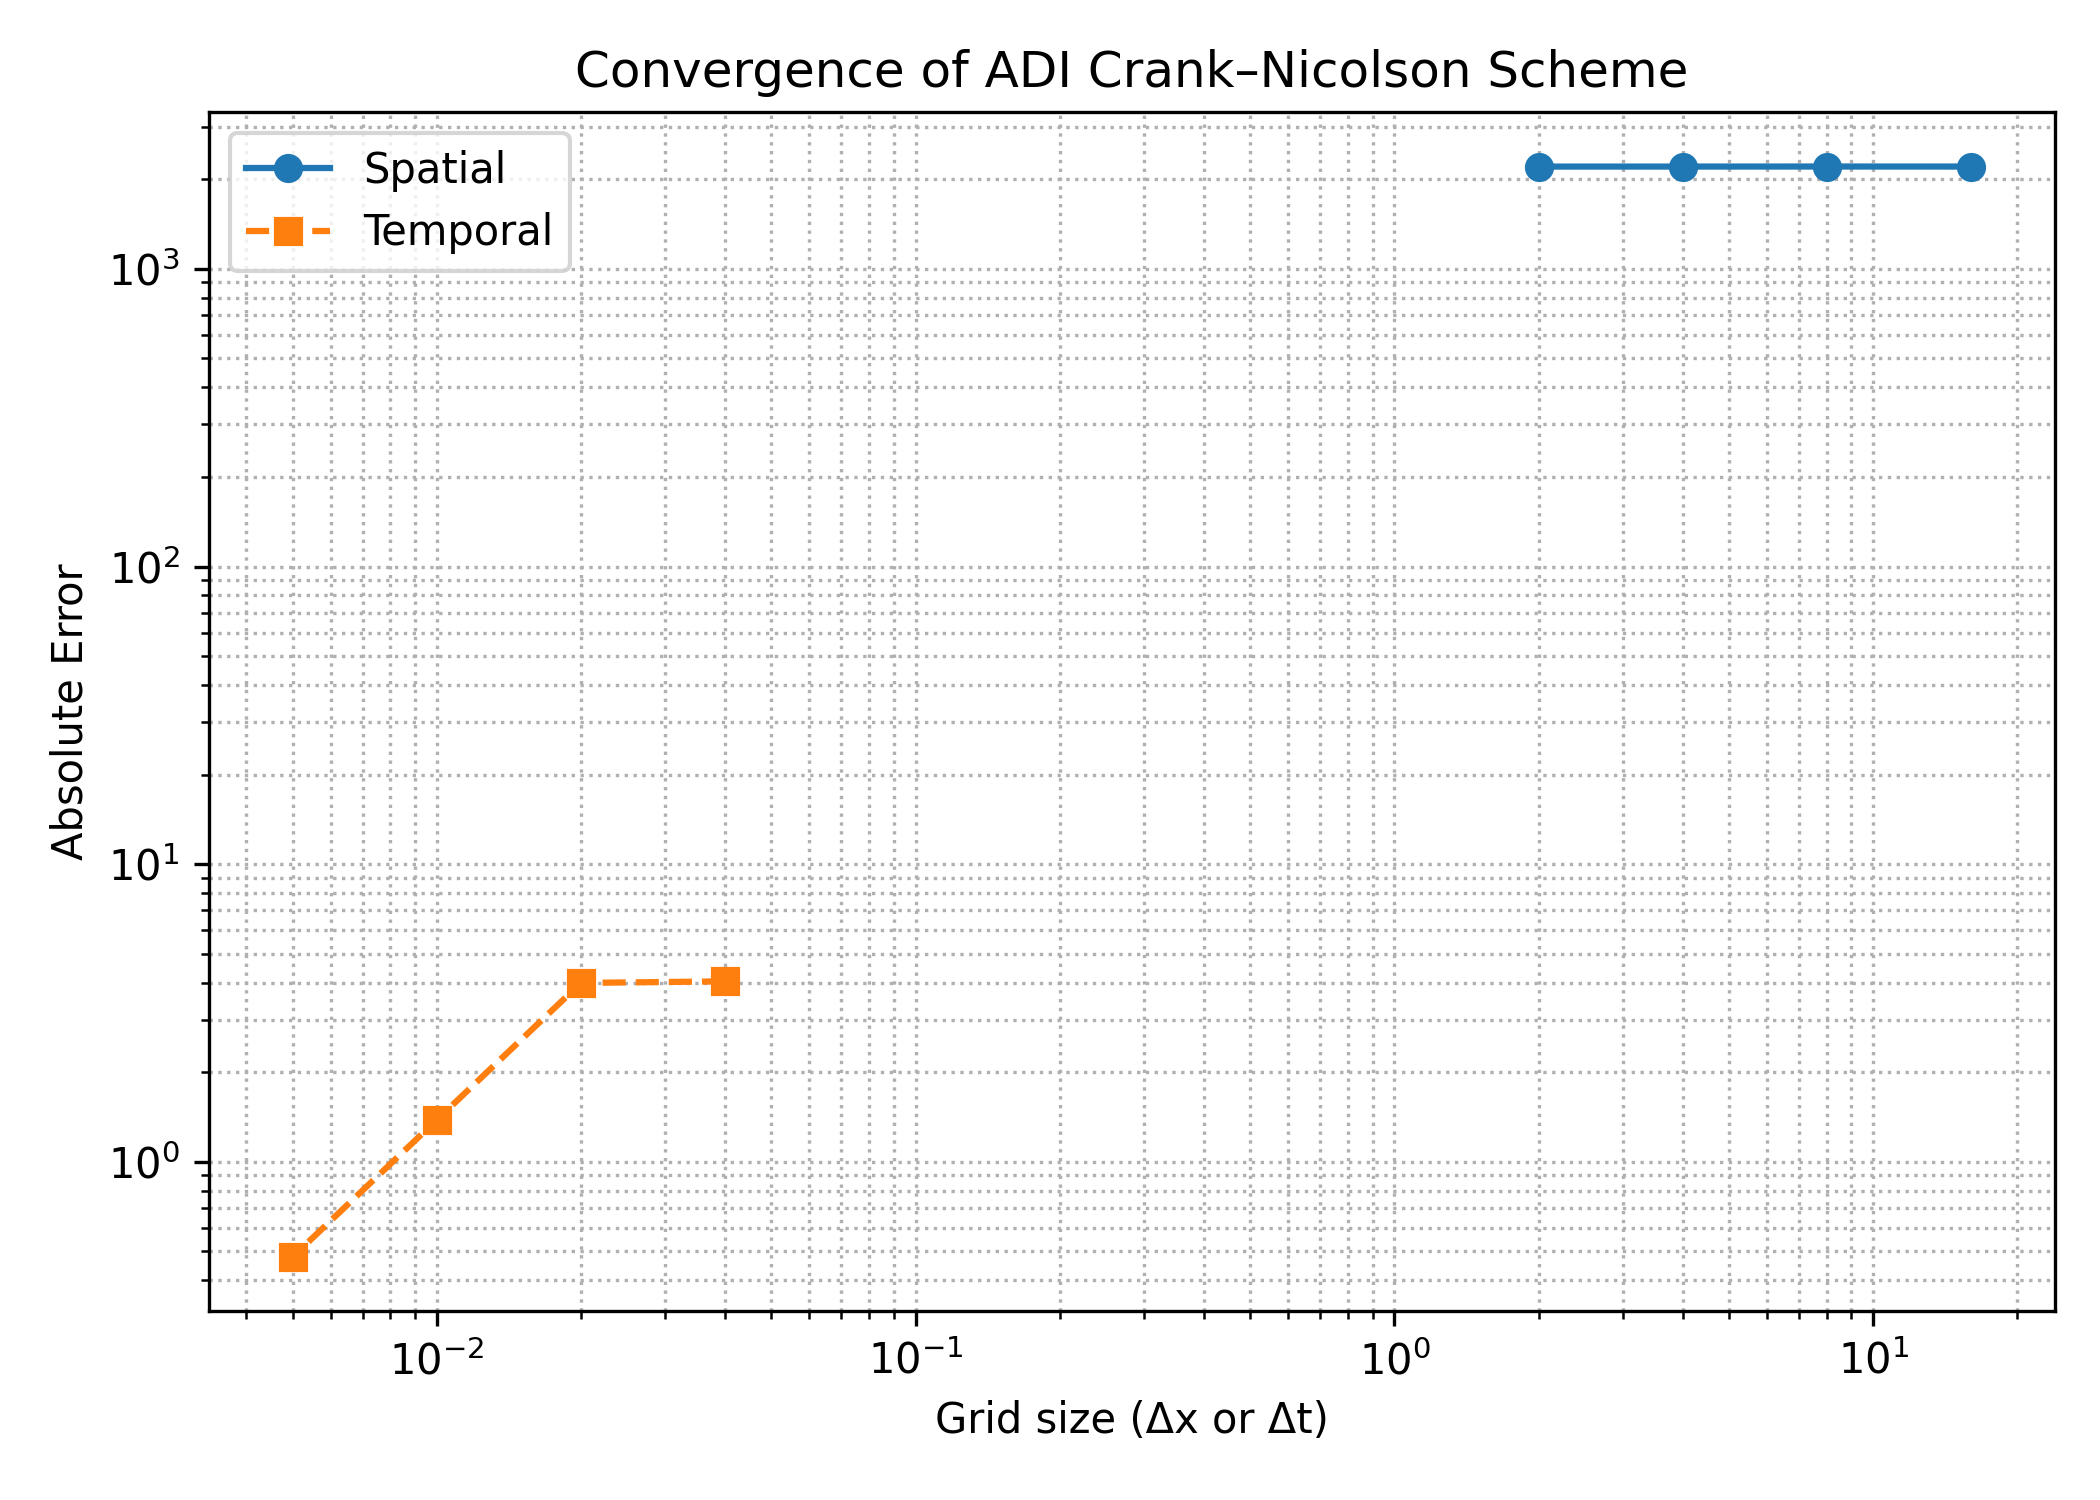
\includegraphics[width=0.75\textwidth]{../plots/asian_adi_convergence.png}
    \caption{Convergence of the ADI Crank–Nicolson scheme for pricing Asian options. Spatial and temporal errors are shown, indicating second-order convergence with respect to time step $\Delta t$ and grid spacing $\Delta x$.}
\end{figure}

\subsection{Runtime vs Accuracy Tradeoff}

Finally, we analyze the efficiency of all solvers. While PDE methods offer superior accuracy per unit time, MC methods offer flexibility for exotic payoffs.

\begin{figure}[H]
    \centering
    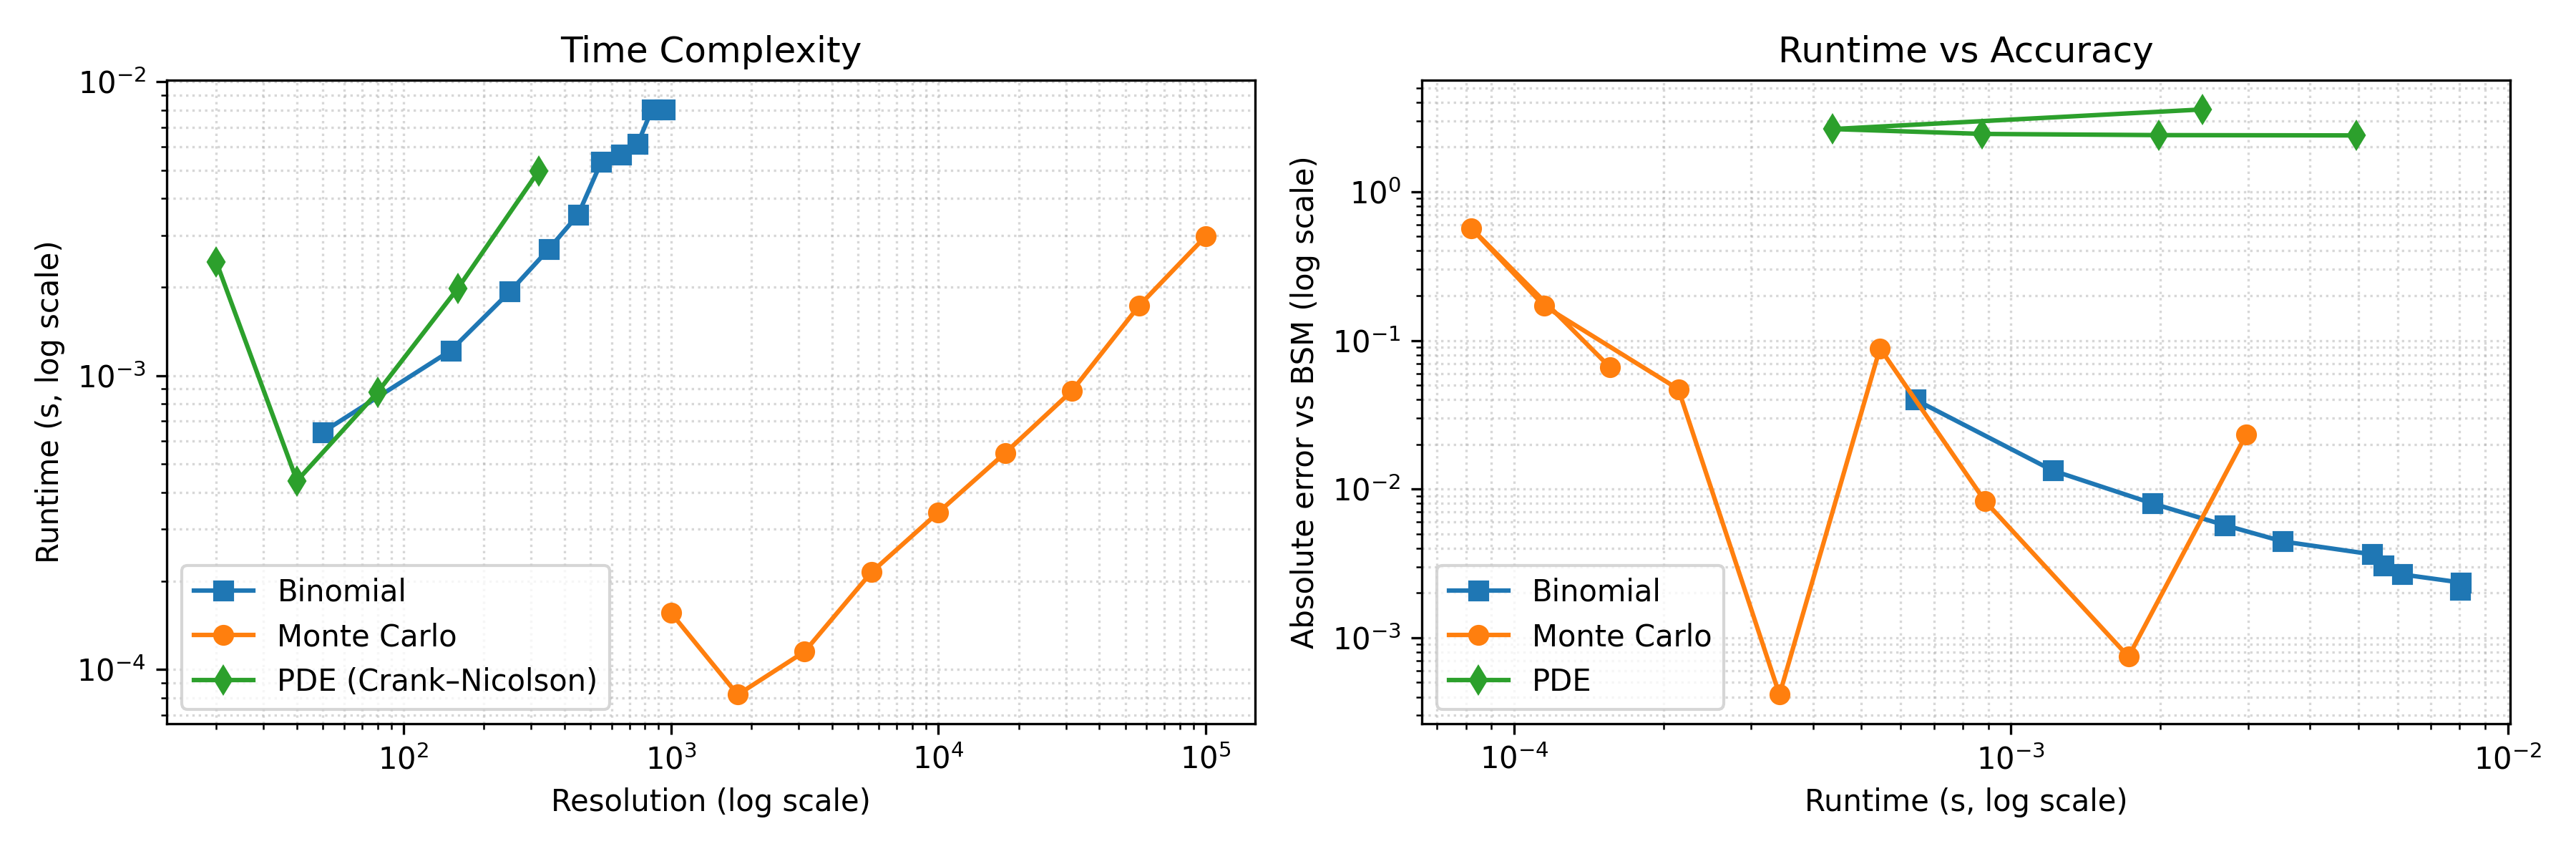
\includegraphics[width=0.95\textwidth]{../plots/error_runtime_comparison.png}
    \caption{Left: Runtime vs resolution (log-log scale) across solvers. Right: Tradeoff between runtime and absolute error vs BSM closed-form. PDE achieves high accuracy rapidly; MC is more computationally expensive; Binomial is slow but reliable.}
\end{figure}
\newpage

\section{Discussion}

\subsection{PDE vs. Monte Carlo Efficiency}
The Crank-Nicolson PDE solver exhibited fast convergence and strong accuracy for European and barrier options. Its implicit time-stepping and stability allowed for efficient pricing under well-defined boundaries. In contrast, Monte Carlo methods were more computationally intensive but offered greater flexibility for path-dependent payoffs such as Asian options.

\subsection{Impact of Variance Reduction}
Variance reduction significantly improved Monte Carlo performance. Antithetic variates helped reduce path noise, control variates using BSM provided analytical guidance, and Sobol sequences accelerated convergence. These techniques were particularly effective in exotic scenarios where standard Monte Carlo would require more simulations.

\subsection{Accuracy and Runtime Trade-offs}
Our runtime vs. error plots showed that PDE methods reached high accuracy faster, making them ideal for vanilla and semi-exotic options. Monte Carlo required longer runtimes for similar precision, but its ability to handle arbitrary payoffs makes it essential when PDEs are impractical.

\subsection{Greeks Estimation for Hedging}
We estimated Delta, Gamma, and Vega using both finite differences and Monte Carlo-based techniques. The pathwise and likelihood ratio methods yielded stable sensitivities, reinforcing their use in risk management. Monte Carlo estimators were especially helpful when analytical Greeks were unavailable.

\subsection{Convergence Behavior}
As expected, Monte Carlo methods showed \( O(1/\sqrt{N}) \) convergence, while PDE methods achieved second-order accuracy. This alignment with theory validated the implementation and highlighted the strengths of each method under increasing computational budget.

\subsection{Summary}
Overall, each method had distinct advantages. PDE solvers are best suited for fast, accurate pricing of options with smooth payoff structures and defined boundaries. Monte Carlo methods, though slower, offer unmatched flexibility and are essential for modeling complex path dependencies.
\newpage

\section{Conclusion and Future Work}

This study developed and analyzed multiple computational frameworks for pricing exotic options, including Monte Carlo simulations with variance reduction, finite difference PDE solvers, and the Black-Scholes analytical formula. Through rigorous experimentation and diagnostics, we evaluated the accuracy, convergence behavior, and computational efficiency of these methods under various market scenarios.

Key contributions include a modular Monte Carlo engine capable of pricing both vanilla and exotic options, a stable Crank-Nicolson PDE solver with early exercise handling, and visual diagnostics for method comparison. Exotic options such as Asian and barrier derivatives were priced using multiple approaches, and their sensitivity profiles were also computed. The use of Sobol sequences and control variates demonstrated significant improvements in convergence and variance reduction.

\textbf{Future work} Future work can extend this framework to American-style and path-dependent options with early exercise features. Additionally, incorporating stochastic volatility models (e.g., Heston model), local volatility surfaces, and machine learning-based regression techniques (e.g., Longstaff-Schwartz) for American Monte Carlo methods could further enhance the pricing toolkit. 

Another key direction is model calibration and backtesting — aligning theoretical models with observed market prices and evaluating historical performance. This would bridge the gap between academic pricing and practical trading applications, making the models more robust and deployment-ready.

\bibliographystyle{plain}
\bibliographystyle{ieeetr}
\bibliography{references}
\newpage

\appendix
\section{Appendix A: Math Derivations}

\subsection{Black-Scholes-Merton (BSM) Formula Derivation}
Assume the underlying asset price follows Geometric Brownian Motion:
\[
dS_t = \mu S_t \, dt + \sigma S_t \, dW_t
\]
Under the risk-neutral measure \(\mathbb{Q}\), this becomes:
\[
dS_t = r S_t \, dt + \sigma S_t \, dW_t^{\mathbb{Q}}
\]
Applying Itô’s Lemma to the option price \(V(S,t)\), we derive the Black-Scholes PDE:
\[
\frac{\partial V}{\partial t} + \frac{1}{2} \sigma^2 S^2 \frac{\partial^2 V}{\partial S^2} + r S \frac{\partial V}{\partial S} - rV = 0
\]
Solving this PDE gives the closed-form price for a European call:
\[
C = S_0 \Phi(d_1) - K e^{-rT} \Phi(d_2)
\]
where:
\[
d_1 = \frac{\ln(S_0 / K) + (r + 0.5 \sigma^2)T}{\sigma \sqrt{T}}, \quad d_2 = d_1 - \sigma \sqrt{T}
\]
and \(\Phi(\cdot)\) is the cumulative distribution function of the standard normal distribution.

\subsection{Monte Carlo Estimator for Option Pricing}
Using risk-neutral valuation:
\[
V_0 = \mathbb{E}^{\mathbb{Q}} \left[ e^{-rT} \cdot \text{Payoff}(S_T) \right]
\]
Approximated via Monte Carlo with \(N\) paths:
\[
\hat{V}_0 = \frac{e^{-rT}}{N} \sum_{i=1}^N \text{Payoff}(S_T^{(i)})
\]

\subsection{Asian Option Payoff (Arithmetic Average)}
For an Asian call option, the arithmetic average payoff is:
\[
\text{Payoff}_{\text{Asian}} = \max\left( \frac{1}{M} \sum_{j=1}^M S_{t_j} - K,\, 0 \right)
\]
where \(t_1, \dots, t_M\) are monitoring times.

\subsection{Barrier Option (Knock-Out Condition)}
For a down-and-out barrier call:
\[
\text{Payoff}_{\text{Barrier}} = 
\begin{cases}
\max(S_T - K, 0) & \text{if } S_t > B \text{ for all } t \in [0, T] \\
0 & \text{otherwise}
\end{cases}
\]

\subsection{Crank-Nicolson Finite Difference Scheme}
The Black-Scholes PDE is discretized using the Crank-Nicolson method:
\[
\frac{V_i^{n+1} - V_i^n}{\Delta t} = \frac{1}{2} \left[ \mathcal{L} V^n + \mathcal{L} V^{n+1} \right]
\]
where the operator \(\mathcal{L}\) is:
\[
\mathcal{L} V_i = \frac{1}{2} \sigma^2 S_i^2 \frac{V_{i+1} - 2V_i + V_{i-1}}{(\Delta S)^2} 
+ r S_i \frac{V_{i+1} - V_{i-1}}{2 \Delta S} - r V_i
\]
This leads to solving a tridiagonal system at each time step.
\newpage

\section{Appendix B: Code Snippets}

\subsection{Black-Scholes Formula Implementation}
\begin{lstlisting}
import numpy as np
from scipy.stats import norm

def black_scholes_price(S, K, T, r, sigma, option_type="call"):
    if T <= 0 or sigma <= 0 or S <= 0 or K <= 0:
        return 0.0

    d1 = (np.log(S / K) + (r + 0.5 * sigma**2) * T) / (sigma * np.sqrt(T))
    d2 = d1 - sigma * np.sqrt(T)

    if option_type == "call":
        return S * norm.cdf(d1) - K * np.exp(-r * T) * norm.cdf(d2)
    elif option_type == "put":
        return K * np.exp(-r * T) * norm.cdf(-d2) - S * norm.cdf(-d1)
    else:
        raise ValueError("option_type must be 'call' or 'put'")
\end{lstlisting}

\vspace{1em}

\subsection{Monte Carlo pricing for European Options}
\begin{lstlisting}
import numpy as np

def mc_european_price(S0, K, r, sigma, T, N_paths=100_000, N_steps=252, 
                      is_call=True, seed=None):
    if seed is not None:
        np.random.seed(seed)

    dt = T / N_steps
    # simulate log returns
    Z = np.random.randn(N_paths, N_steps)
    increments = (r - 0.5*sigma**2)*dt + sigma*np.sqrt(dt)*Z
    logS = np.cumsum(increments, axis=1)
    ST = S0 * np.exp(logS[:,-1])

    # payoff
    if is_call:
        payoff = np.maximum(ST - K, 0.0)
    else:
        payoff = np.maximum(K - ST, 0.0)

    discounted = np.exp(-r*T) * payoff
    price = discounted.mean()
    stderr = discounted.std(ddof=1) / np.sqrt(N_paths)
    ci_95 = 1.96 * stderr
    return price, ci_95
\end{lstlisting}

\vspace{1em}

\subsection{Crank-Nicolson PDE Solver}
\begin{lstlisting}
import numpy as np
from scipy.stats import norm
from scipy.linalg import solve_banded

def crank_nicolson(S0, K, r, sigma, T, Smax=300, M=100, N=100, option_type='call'):
    dS = Smax / M
    dt = T / N
    S = np.linspace(0, Smax, M+1)
    V = np.maximum(0, S - K) if option_type == 'call' else np.maximum(0, K - S)

    alpha = 0.25 * dt * (sigma ** 2 * (np.arange(M+1)) ** 2 - r * np.arange(M+1))
    beta  = -dt * 0.5 * (sigma ** 2 * (np.arange(M+1)) ** 2 + r)
    gamma = 0.25 * dt * (sigma ** 2 * (np.arange(M+1)) ** 2 + r * np.arange(M+1))

    A = np.zeros((3, M-1))
    B = np.zeros((3, M-1))
    for i in range(1, M):
        A[0, i-1] = -alpha[i]
        A[1, i-1] = 1 - beta[i]
        A[2, i-1] = -gamma[i]

        B[0, i-1] = alpha[i]
        B[1, i-1] = 1 + beta[i]
        B[2, i-1] = gamma[i]

    for _ in range(N):
        rhs = B[0] * V[0:M-1] + B[1] * V[1:M] + B[2] * V[2:M+1]
        V[1:M] = solve_banded((1, 1), A, rhs)
        V[0] = 0
        V[M] = Smax - K * np.exp(-r * (T - _ * dt)) if option_type == 'call' else K * np.exp(-r * (T - _ * dt))

    price = np.interp(S0, S, V)
    return price
\end{lstlisting}

\end{document}